\section{kmfc: un générateur de code}

Après m'être familiarisé avec le système \emph{Contiki}, le paradigme du \emph{model@runtime} et son implémentation \emph{Kevoree-C} j'ai pu commencer l'objectif principal de mon stage, à savoir produire dynamiquement les parties critiques de \emph{Kevoree-C} à partir d'un méta-modèle \emph{Kevoree}.

\subsection{Intérêt de générer du code}

Comme décrit en partie \ref{kevoree} l'actuelle version de \emph{Kevoree-C} a été écrite manuellement. En plus d'avoir une série d'inconvénients, l'écriture manuelle a également quelques avantages que la ré-écriture générique se devra d'essayer de conserver.

Ces inconvénients sont en partie les mêmes que ceux détaillés dans la partie \ref{parser-spécif} et son avantage principal découle de ces défauts, en étant si spécifique à la version du méta-modèle lu et à la structure de données, le programme final est très performant. L'objectif va être de produire du code le plus optimisé possible même s'il sera théoriquement difficile d'atteindre ce même niveau. Ici la notion d'optimisation est subjective, elle consiste plus à évaluer la manière dont le stockage des données est réalisés, les éventuelles redondances d'information et la complexité algorithmique des sections critiques.

Il est par exemple évident que le code source du générateur de code doit privilégier la lisibilité à la rapidité d'exécution.

\subsection{\label{mm-kevoree}Méta-modèle \emph{Kevoree}}

Le méta-modèle de \emph{Kevoree} peut être représenté de la même manière qu'un méta-modèle \emph{EMF}, \emph{Eclipse}\cite{eclipse} et en particulier sa version \emph{Eclipse Modeling Tools}\cite{eclipse-emf} peut être utilisé pour l'afficher. 

L'extrait de diagramme en Figure \ref{kevoree-cd}, page \pageref{kevoree-cd} et l'Annexe \ref{kevoree-full-cd} montrent que les classes possèdent généralement peu d'attributs primitifs. Ils permettent également de remarquer que de nombreuses classes implémentent l'interface \emph{NamedElement} et obtiennent donc un attribut \emph{name} et que toutes les classes sont référencées directement ou indirectement par la classe \emph{ContainerRoot}.

\begin{figure}[ht!]
\centering
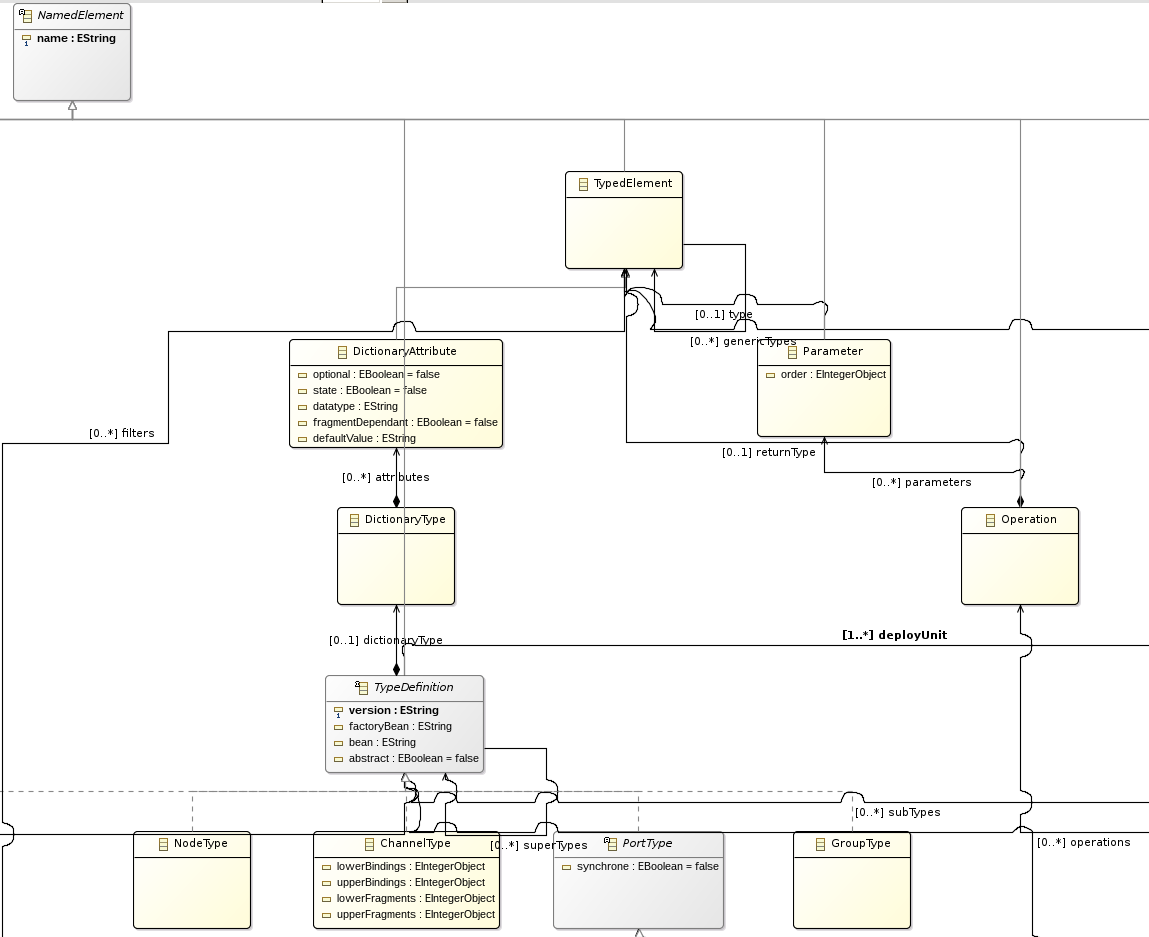
\includegraphics[scale=0.4]{images/kevoree-cd.png}
\caption{Extrait du méta-modèle de Kevoree v4 écrit en KMF2}
\label{kevoree-cd}
\end{figure}

\subsection{Structure de \emph{Kevoree}}

Pour résumer, \emph{Kevoree-c} est composé d'une structure de données détaillée en section \ref{mm-kevoree}, d'outils de manipulation pour permettre la sérialisation/désérialisation, comparaison de modèles et permettre l'adaptation suite au calcul de ses différences.

\subsection{Flux de travail}

La figure \ref{workfow} en page \pageref{workfow} résume les différentes étapes jusqu'à la création du nouveau firmware et l'utilisation du méta-modèle \emph{Kevoree-c} et du modèle représentant les instances et leurs modules. Le compilateur utilisé pour cibler une machine personnelle est \emph{gcc} et pour cibler les nœuds \emph{m3} sa version de compilation croisée \emph{arm-none-eabi-gcc}.

\begin{figure}[ht!]
\centering
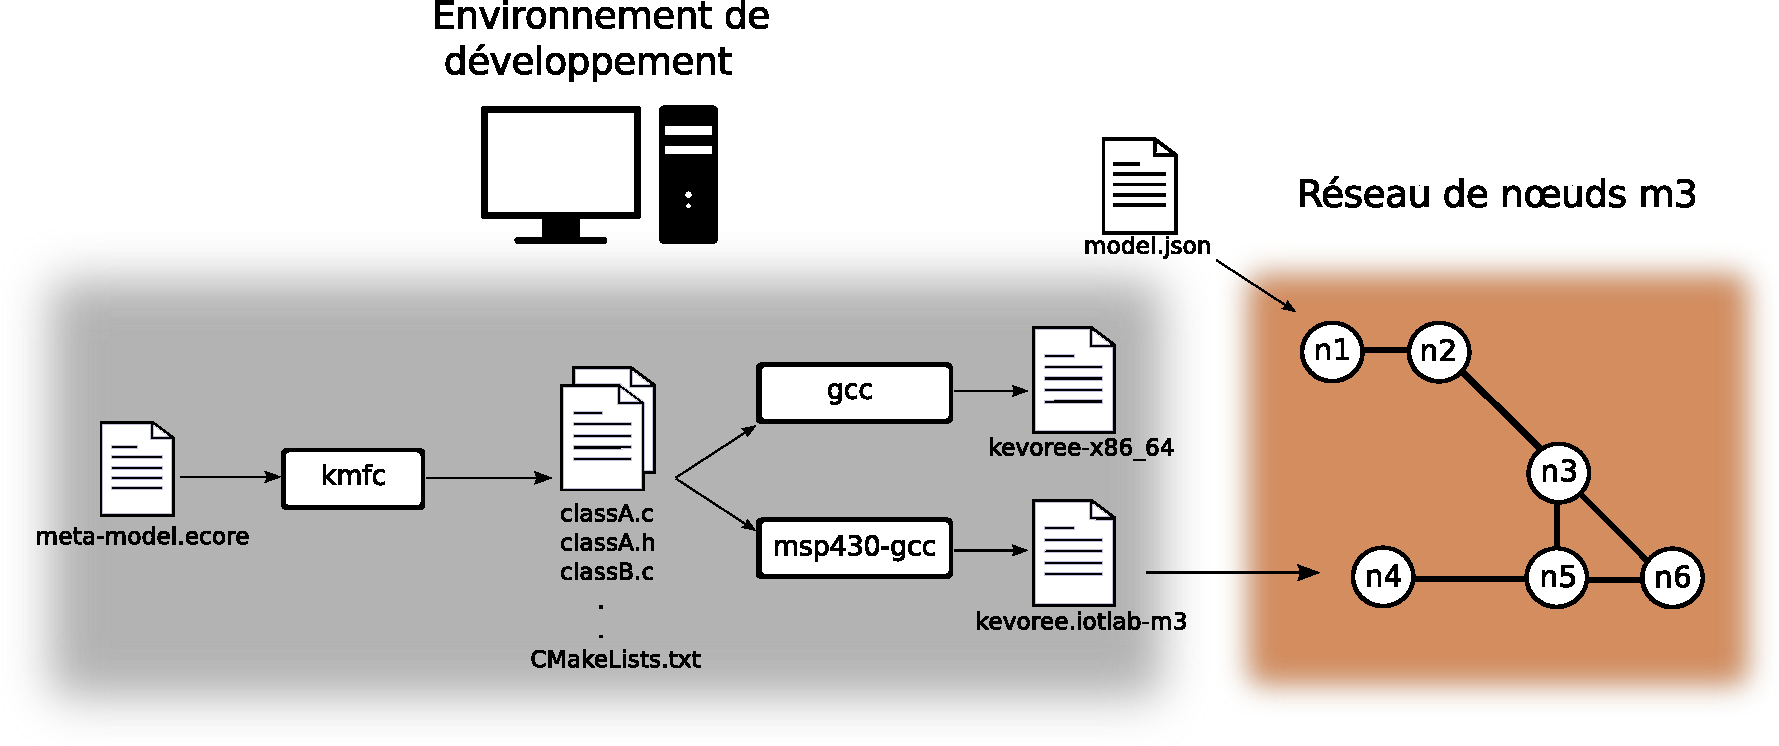
\includegraphics[scale=0.55]{images/workflow-schema/workflow.pdf}
\caption{Flux de travail du développement au déploiement du nouveau firmware.}
\label{workfow}
\end{figure}

\subsection{\label{kmfcpp}kmfcpp}

Avant de commencer mon générateur de code \johann et \paco m'ont indiqué de regarder la version \emph{C++}\footnote{https://github.com/kevoree/kmfcpp} de \emph{KMF}. Bien que le langage de destination ne soit pas le même le format du méta-modèle d'entrée est identique, c'est une partie qui peut donc être réutilisée.

Le langage \emph{C++} permet nativement beaucoup de mécanismes utiles à la représentation d'une telle structure de données, à savoir :

\begin{itemize}
\item le paradigme d'orienté objet qui permet une encapsulation des attributs et des méthodes,
\item l'héritage et le polymorphisme, qui sont utilisés dans le méta-modèle,
\item une simplification de la gestion de la mémoire allouée dynamiquement, avec les destructeurs de classes
\end{itemize}

Ces fonctionnalités natives font que \emph{kmfcpp} ne génère que peu de code et peut le faire en ne parcourant le méta-modèle qu'une seule fois et en produisant directement le code \emph{C++} équivalent.

Pour générer du code \emph{kmfc} utilise le framework \emph{Velocity}\cite{velocity}, il permet de créer des templates de texte contenant des variables ou des structures de contrôle qui seront évaluées et remplacées lors du parsing du méta-modèle.

L'utilisation d'un moteur de template permet de séparer la logique algorithmique du générateur du code même généré. La lisibilité en est grandement améliorée.

\subsubsection{L'utilisation de template}

Comme visible sur le Listing \ref{velocity} en page \pageref{velocity} la syntaxe de \emph{Velocity} permet de gagner en lisibilité. Les instructions de pré-processeur \emph{C}, par exemple lignes 1, 3 et 4, doivent être explicitement ignorées en étant encadrées par \texttt{\#[[ ]]\#}, \texttt{\#include} étant également une instruction \emph{Velocity}.

Les variables \emph{Java} sont référencées en écrivant \texttt{\$variable}, par exemple ligne 14. Une variable de type primitif sera directement affiché, les objets se verront automatiquement appelé leur méthode \texttt{toString()}.

\emph{Velocity} permet également d'appeler les méthodes des objets, comme en ligne 9.

Pour finir, les structures de contrôle permettent de calculer uniquement une liste du côté \emph{Java} et de la passer à \emph{Velocity} qui se contentera de la parcourir, comme visible en ligne 24 à 26.

\lstset{
 language=C,
 captionpos=b,
 otherkeywords={foreach, end, in, include},
 numbers=left,
 caption={Fichier testSource.vm permettant de générer un fichier de test unitaire.}
}

\begin{lstlisting}[frame=single, label={velocity}]
#[[#include "]]#$name#[[Test.h"]]#

#[[#include <stdlib.h>]]#
#[[#include <check.h>]]#

#foreach ($test in $testSuite.keySet())
START_TEST ($test)
{
$testSuite.get($test)
}
END_TEST

#end
Suite* $name#[[_suite(void)]]#
{
	Suite *s;
	TCase *tc_core;

	s = suite_create("$name");

	/* Core test case */
	tc_core = tcase_create("Core");

#foreach( $test in $testSuite.keySet() )
	tcase_add_test(tc_core, $test);
#end
	suite_add_tcase(s, tc_core);

	return s;
}
\end{lstlisting}

\subsection{Un vrai compilateur}

Les premières versions de \emph{kmf} adoptaient plus une logique de transcription de méta-modèles vers le langage \emph{C}, à l'image de \emph{kmfcpp} la génération de code était réalisée directement pendant le parcours du méta-modèle d'entrée.

Un compilateur se différencie par sa représentation intermédiaire. Le travail du compilateur est alors séparé en deux parties, une face avant et une face arrière. La face avant est chargée de lire le langage d'entrée, ici un méta-modèle et d'en construire une représentation intermédiaire propre au compilateur. La face arrière se charge de générer du code, ici du \emph{C} à partir de cette représentation.

La représentation intermédiaire permet de séparer les préoccupations et offre de nombreux avantages.

Parmi ces avantages, les suivants peuvent nous concerner :
\begin{itemize}
\item il est plus aisé de corriger ou comment le modèle est lu ou comment le code \emph{C} est généré,
\item l'optimisation s'effectuera sur la représentation intermédiaire et ne sera pas dépendante des formats lus et produits,
\item lire un nouveau format de méta-modèle n'impacte qu'au maximum la moitié du code,
\item de même que cibler un nouveau langage ou une variante de \emph{C}
\end{itemize}

En plus d'un enseignement de Compilation suivi à l'\univname je me suis documenté\cite{aho2007compilateurs}, \cite{Appel2003MCI599718} durant la rédaction de ce compilateur.

\subsection{Générer une structure de données}

La première étape est donc, petit à petit, comprendre la manière dont \emph{Kevoree-c} a été écrit pour pouvoir «lier» les parties de code au méta-modèle. De manière, générale pour implémenter les paradigmes nécessaires tels que détaillés dans la section \ref{kmfcpp} en optimisant la taille du binaire produit l'utilisation de pointeurs sur variables et sur fonctions est primordiale.

\subsubsection{Construction d'une classe}

Une classe du méta-modèle est représenté par un fichier \texttt{.h} permettant d'exposer des informations au reste du compilateur et un fichier \texttt{.c} contenant entre autre l'implémentation des méthodes métiers.

Une classe \emph{C} est donc composée de :
\begin{itemize}
\item une \texttt{struct} pour stocker tous les attributs,
\item une autre \texttt{struct} représentant une \emph{Table Virtuelle}. Elle contient toutes les fonctions que la classe est censée posséder sous forme de pointeurs sur fonctions.
\end{itemize}

La \texttt{struct} des attributs possède un pointeur sur la \texttt{struct} représentant la table virtuelle, de cette manière elle peut représenter la classe et pour une question de clarté, porte son nom.

La contrainte est de connaître la taille de chaque attribut au moment de la compilation. Les types primitifs ne posent pas de problèmes pour avoir un équivalent en \emph{C}, les relations unaires sont représentés par un pointeur sur la \texttt{struct} des attributs de la classe voulue. En revanche les relations multiples du méta-modèle du type \texttt{0-*} produirait un tableau de taille variable, la solution est de gérer cette mémoire de façon dynamique. Cette préoccupation a déjà été résolue dans \emph{Kevoree-C} en développant la structure de données \texttt{map\_t}.

\subsubsection{Gestion de l'héritage}

Grâce à ces deux \texttt{struct} l'héritage est géré de manière simple, si une classe \texttt{B} hérite d'une classe \texttt{A} alors tous les attributs de \texttt{A} seront copiés dans la \texttt{struct} de \texttt{B}.

Pour l'appel de fonctions définies dans une classe mère plusieurs approches sont possibles.

La première est d'hériter des pointeurs de fonctions parents en les copiant et en les faisant pointer sur le code contenu dans les classes mères en passant par l'attribut \texttt{super} pointant sur la classe mère. De cette manière le code de la méthode n'est pas dupliqué mais le compilateur ne peut déterminer l'emplacement de code à la compilation et ne peut pas initialiser la \texttt{struct} en la laissant constante. C'est l'approche utilisée actuellement dans \emph{kmfc}.

Une autre approche est d'ajouter des fonctions qui vont elles se contenter d'appeler le code parent. C'est l'approche utilisée dans la version de \emph{Kevoree-C}.

\subsubsection{Gestion du polymorphisme}

Le langage \emph{C} offre une possibilité d'outre passer la vérification des types des pointeurs. En utilisant la notation \texttt{void*} et des casts il est possible d'utiliser le polymorphisme.

L'utilisation de \texttt{void*} pour désigner un espace mémoire rend difficile la relecture du code, l'avantage réside dans le fait que le code est généré et ne doit en théorie pas être relu ou modifié directement. Les modifications sont à faire dans le générateur, où le code est isolé et le rôle de chaque variable facile à déterminer.

\subsubsection{Exemple d'implémentation}

L'annexe \ref{dico-struct} en page \pageref{dico-struct} résume l'héritage des attributs, leur typage, la gestion de la table virtuelle et des déclarations des signatures de fonction.

\subsubsection{Générer des tests unitaires}

En plus de générer une structure de données j'ai estimer que générer du code unitaire pour cette structure avait des avantages. Pour chaque méthode de chaque classe je génère au moins un test unitaire.

En plus de vérifier que l'appel des méthodes modifient l'état de l'objet leur rôle est surtout de s'assurer que les appels peuvent être réalisés. Un appel de pointeur de fonctions mal initialisé résulterait par un échec du test.

Aucun test n'était réalisé sur \emph{Kevoree-C}.

\subsection{Générer des outils de manipulation}

En plus de la structure de données il faut pouvoir effectuer les actions nécessaires au paradigme du \emph{model@runtime}.

La sérialisation des instances courantes est possible par simple appel à une méthode de la classe \emph{ContainerRoot}, l'appel est ensuite propagé aux objets référencés, comme implémenté dans \emph{Kevoree-C}. Une approche utilisant le patron de conception Visiteur\cite{freeman2004head} a été implémenté mais le format JSON demande un traitement particulier pour les éléments en début et fin de liste alors que Visiteur demande à ce que chaque objet effectue son action indépendamment. Par exemple une liste comment par un \texttt{[}, finit par \texttt{]} et chaque élément, sauf le dernier, est suivi d'une virgule.

La désérialisation est pensée de manière totalement différente de celle implémentée dans \emph{Kevoree-C} pour palier à ces défauts, voir section \ref{}. Quelques fonctions génériques telles que \texttt{parseObject} et \texttt{parseArray} sont appelées en fonction du contexte pour récupérer les informations voulues du fichier JSON. Le contexte, les attributs attendus et la hiérarchie à parcourir, sont définis par un ensemble de tables tel que le Listing \ref{deserial}.

\lstset{
 language=C,
 captionpos=b,
 otherkeywords={},
 numbers=left,
 caption={Exemple de structure permettant de connaître le schéma de désérialisation.}
}

\begin{lstlisting}[frame=single, label={deserial}]
const struct at NodeNetwork_Attr[NodeNetwork_NB_ATTR] = {
{"eClass", doNothing, PRIMITIVE_TYPE, PRIMITIVE_TYPE},
{"generated_KMF_ID", NodeNetworkSetgenerated_KMF_ID, NODENETWORK_TYPE, PRIMITIVE_TYPE},
{"link", parseArray, NODENETWORK_TYPE, NODELINK_TYPE},
{"initBy", NodeNetworkSetinitBy, NODENETWORK_TYPE, CONTAINERNODE_TYPE},
{"target", NodeNetworkSettarget, NODENETWORK_TYPE, CONTAINERNODE_TYPE},
};
\end{lstlisting}

L'intérêt est de n'écrire le nom de l'attribut qu'une fois.
Un pointeur de fonctions lui est associé et est appelé lorsque cet attribut est rencontré ainsi que deux types énumérés pour définir un contexte, le premier identifie la classe à laquelle l'attribut appartient, le second le type de l'objet à lire s'il s'agit d'un lien multiple.

Les mécanismes de comparaison et d'adaptation ne représentent pas la partie critique de \emph{Kevoree-C}, leurs algorithmes seront donc repris et incorporés à \emph{kmfc}.

\subsection{Générer le reste}

Pour avoir un projet complet et fonctionnel d'autres fichiers doivent également être inclus ou générés. Il s'agit de fichier correspondant à des types tels que \texttt{map\_t} ou pour gérer le format JSON. Ces fichiers sont simplement ajoutés au code généré.

Des fichiers lanceurs, contenant une méthode \texttt{main}, sont également copiés, il me permette de développer une fonctionnalité d'abord sur quelques classes choisies avant de l'ajouter au compilateur et de gérer l'ensemble des classes couvertes par le méta-modèle.

D'autres fichiers sont nécessaires à la compilation du projet. La compilation est assistée par \emph{cmake}\cite{cmake} pour gérer facilement la production de différents exécutables : un pour chaque fichier contenant une méthode \texttt{main}, un pour lancer la suite de tests. Cmake permet de n'inclure les tests que dans l'exécutable lançant les tests.